\documentclass[12pt]{article}
\usepackage[utf8]{inputenc}
\usepackage{amsmath,amssymb,amsthm}
\usepackage{graphicx}
\usepackage{hyperref}

\title{FM3817B Assignment 1}
\author{Patrick Connors \\ Student Number: 251313609}
\date{\today}

\begin{document}

\maketitle

\section*{General Information}
\begin{itemize}
    \item \textbf{Created by:} Yifan Li
    \item \textbf{Due Date:} January 28, 2025, 11:55 pm
\end{itemize}

\subsection*{Instructions (Excerpted)}
\begin{itemize}
    \item Questions with bonus points: If you do it correctly, you will get the bonus points (until reaching full scores). Otherwise, no deduction. So feel free to try them out.
    \item More questions may be added progressively; the assignment will be finalized by January 21, 2025.
    \item You must submit a single PDF file through Gradescope. Format your submission carefully, assigning pages to corresponding questions.
    \item Late submissions are \textbf{not} accepted.
    \item You may discuss with classmates, but you must write and submit your own work. Scholastic offences are taken seriously.
\end{itemize}

\section*{Question 1 (6 pts)}
\textbf{Prospect Theory Utility Function.} Consider the utility function:
\[
U(x) = 
\begin{cases} 
x^\alpha, & \text{if } x \ge 0,\\
-\lambda \,(-x)^\alpha, & \text{if } x < 0,
\end{cases}
\]
where \(x\) represents gain or loss, and the parameters are set as \(\alpha = 0.9\) and \(\lambda = 2\).

\begin{enumerate}
    \item[(a)] Compute \(U'(x)\) for \(x > 0\) and \(x < 0\). Discuss whether the function increases or decreases on \(x > 0\) and on \(x < 0\).

    \item[(b)] Compute \(U''(x)\) for \(x > 0\) and \(x < 0\). Discuss whether it is convex or concave on \(x > 0\) and on \(x < 0\).

    \item[(c)] Determine if \(U\) is continuous at \(x = 0\). (Yes or No.) Determine if \(U\) is differentiable at \(x = 0\). (Yes or No.)
\end{enumerate}

\vspace{1cm}

\noindent \textbf{Answer:}

\bigskip

\noindent
\textbf{(a) First Derivative and Monotonicity}

\[
U(x) = 
\begin{cases}
x^\alpha, & x \ge 0,\\
-\lambda\,(-x)^\alpha, & x < 0.
\end{cases}
\]
\[
\alpha = 0.9, \quad \lambda = 2.
\]

\paragraph{Case 1: \(x>0\).} 
\[
U(x) = x^\alpha 
\quad \Longrightarrow \quad
U'(x) = \frac{d}{dx}\bigl(x^\alpha\bigr) = \alpha\, x^{\alpha - 1}.
\]
Since \(\alpha = 0.9\) and \(x>0\), we have \(x^{\alpha-1} = x^{-0.1} > 0\). Thus
\[
U'(x) = 0.9\, x^{-0.1} > 0,\quad \text{so }U(x)\text{ is increasing on }(0,\infty).
\]

\paragraph{Case 2: \(x<0\).} 
\[
U(x) = -\lambda\,(-x)^\alpha
\quad \Longrightarrow \quad
U'(x) = -\lambda \,\frac{d}{dx}\bigl[(-x)^\alpha\bigr].
\]
Since \(\frac{d}{dx}(-x)^\alpha = \alpha\,(-x)^{\alpha-1}\, \frac{d}{dx}(-x) = \alpha\,(-x)^{\alpha-1} \,(-1)\),
\[
U'(x) 
= -\lambda \,\Bigl[\alpha\,(-x)^{\alpha-1}\,(-1)\Bigr]
= \lambda\,\alpha\,(-x)^{\alpha-1}, \quad x<0.
\]
For \(x<0\), \(-x>0\), so \((-x)^{\alpha-1} >0\). Hence
\[
U'(x) = 2 \times 0.9 \times (-x)^{-0.1} = 1.8\,(-x)^{-0.1} >0,
\]
which means \(U(x)\) is also increasing on \((-\infty,0)\).

\bigskip
\noindent
\textbf{(b) Second Derivative and Convexity/Concavity}

\paragraph{Case 1: \(x>0\).} 
Starting from \(U'(x) = \alpha\, x^{\alpha-1}\):
\[
U''(x) = \alpha \,\frac{d}{dx}\bigl(x^{\alpha - 1}\bigr) 
= \alpha\,(\alpha - 1)\,x^{\alpha - 2}.
\]
With \(\alpha=0.9\), we have \(\alpha - 1 = -0.1\), so
\[
U''(x) = 0.9 \times (-0.1)\, x^{-0.1 -1}
= -0.09\, x^{-1.1}, \quad x>0.
\]
Because \(x^{-1.1}>0\), \(U''(x)<0\). Hence \(U\) is \emph{concave} for \(x>0\).

\paragraph{Case 2: \(x<0\).} 
Starting from \(U'(x) = \lambda \,\alpha\,(-x)^{\alpha - 1}\):
\[
U''(x) 
= \lambda\,\alpha \,\frac{d}{dx}\bigl[(-x)^{\alpha-1}\bigr].
\]
Again, 
\[
\frac{d}{dx}\bigl[(-x)^{\alpha-1}\bigr]
= (\alpha-1)\,(-x)^{\alpha-2}\,\frac{d}{dx}(-x) 
= (\alpha-1)\,(-x)^{\alpha-2}\,(-1).
\]
Thus
\[
U''(x) 
= \lambda\,\alpha\, (\alpha-1)\,(-x)^{\alpha-2} \times (-1)
= -\,\lambda\,\alpha\,(\alpha-1)\,(-x)^{\alpha-2}, \quad x<0.
\]
Plug in \(\alpha=0.9,\;\lambda=2\). Then \(\alpha-1=-0.1\), so
\[
U''(x) 
= -\,2 \times 0.9 \times (-0.1)\,(-x)^{-0.1-1}
= 2 \times 0.9 \times 0.1 \,(-x)^{-1.1}
= 0.18\,(-x)^{-1.1}.
\]
That is \(>0\) for all \(x<0\). Hence \(U\) is \emph{convex} on \((-\infty,0)\).

\bigskip
\noindent
\textbf{(c) Continuity and Differentiability at \(x=0\)}

\paragraph{Continuity at \(x=0\).}
\[
\lim_{x \to 0^+}U(x) = \lim_{x\to 0^+} x^\alpha = 0,\qquad
\lim_{x \to 0^-}U(x) = \lim_{x\to 0^-} -\lambda\,(-x)^\alpha = -\,2\times 0 = 0,
\]
and \(U(0)\) can be taken as \(0^\alpha = 0\). Both one-sided limits agree with the value at 0, so \(\,U\) is \emph{continuous} at \(x=0\).  
\(\boxed{\text{Yes, it is continuous at } x=0.}\)

\paragraph{Differentiability at \(x=0\).}
Consider the \emph{right-hand} derivative:
\[
U'(0^+) = \lim_{x\to 0^+} \alpha\,x^{\alpha-1} 
= 0.9 \,\lim_{x\to 0^+} x^{-0.1} 
= +\infty.
\]
The \emph{left-hand} derivative:
\[
U'(0^-) 
= \lim_{x\to 0^-} \lambda\,\alpha\,(-x)^{\alpha-1}
= 1.8 \,\lim_{x\to 0^-} (-x)^{-0.1}
= +\infty.
\]
Neither side yields a finite derivative. Thus the function does \emph{not} have a well-defined (finite) slope at \(x=0\).  
\(\boxed{\text{No, it is not differentiable at }x=0.}\)

\begin{figure}[htbp]
    \centering
    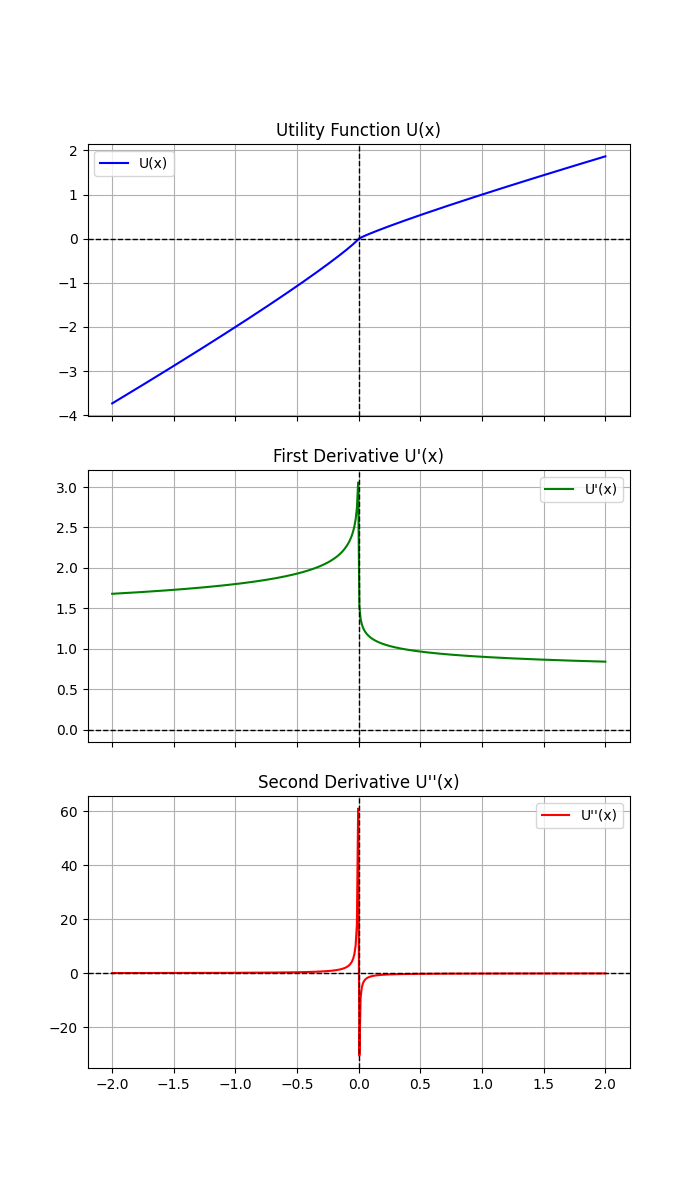
\includegraphics[width=0.7\textwidth]{q1.png}
    \caption{Graphs of \(U(x)\) and its first two derivatives.}
    \label{fig:my_label}
\end{figure}

\newpage

\section*{Question 2 (12 pts)}
\textbf{Set Analysis.} Consider the set \(S = [1, 2) \cup (2, 3]\). Answer the following:

\begin{enumerate}
    \item[(a)] Is \(S\) a closed set? (Yes or No) Why?
    
    \textbf{Answer:} The set
    \[
    S \;=\; [1,2) \;\cup\; (2,3]
    \]
    is \textbf{not} closed.
    
    \hrulefill
        
    We use the given definition of a closed set:
    
    \begin{quote}
    A set \( S \subset \mathbb{R} \) is closed if and only if for \textit{every} convergent sequence \( \{x_n\} \subset S \), the limit of that sequence also lies in \( S \).
    \end{quote}
    
    To show that \( S \) is \textit{not} closed, it suffices to exhibit \textbf{one} convergent sequence entirely contained in \( S \) whose limit does \textit{not} belong to \( S \).
    
    \hrulefill
    
    
    \begin{enumerate}
        \item Observe that \( S \) is the union of the two intervals:
        \[
        [1,2) \quad \text{and} \quad (2,3].
        \]
        Notice that the number \( 2 \) is \textit{excluded} from both intervals:
        \[
        2 \notin [1,2) 
        \quad \text{and} \quad 
        2 \notin (2,3].
        \]
        Hence, \( 2 \notin S \).
        
        \item Consider the sequence \( \{x_n\} \) defined by  
        \[
        x_n \;=\; 2 - \tfrac{1}{n} \quad (n = 1, 2, 3, \dots).
        \]
        
        \item \textbf{Check that \( x_n \) lies in \( S \) for all \( n \):}  
        \begin{itemize}
            \item For each \( n \),
            \[
            2 - \tfrac{1}{n} < 2,
            \]
            which means \( x_n < 2 \).
            
            \item Also, \( 2 - \tfrac{1}{n} \geq 1 \) for all \( n \geq 1 \).
            
            \item Therefore,
            \[
            1 \;\leq\; 2 - \tfrac{1}{n} \;<\; 2,
            \]
            so \( x_n \in [1,2) \). Since \( [1,2) \subset S \), we have \( x_n \in S \) for \textit{every} \( n \).
        \end{itemize}
        
        \item \textbf{Determine the limit of \( \{x_n\} \)}:  
        \[
        \lim_{n \to \infty} \Bigl(2 - \tfrac{1}{n}\Bigr) \;=\; 2.
        \]
        
        \item \textbf{Check if the limit \( 2 \) belongs to \( S \)}:  
        \begin{itemize}
            \item We already noted that \( 2 \notin S \).
        \end{itemize}
    \end{enumerate}
    
    Thus, we have constructed a sequence \( \{x_n\} \subset S \) which converges to a point (\( 2 \)) \textit{outside} of \( S \).
    
    \hrulefill
    
    \subsection*{Conclusion}
    
    Because there exists at least one sequence \( \{x_n\} \subset S \) converging to a limit that is not in \( S \), \( S \) fails the criterion for being a closed set. Therefore,
    
    \[
    \boxed{ S \text{ is not closed.} }
    \]
    \item[(b)] Is \(S\) an open set? (Yes or No) Why? (Please provide two different pieces of evidence.)
    \item[(c)] Is \(S\) a convex set? (Yes or No) Why?
    \item[(d)] If your previous answer is No, what is the simplest way to modify \(S\) such that the new set \(S^*\) is convex? (Hint: there is a unique answer involving only a single point.)
    \item[(e)] For this new set \(S^*\), show that it is indeed a convex set.
\end{enumerate}

\noindent \textbf{Answer:}
\vspace{3cm}

\newpage

\section*{Question 3}
\textbf{Cobb-Douglas Utility Function.} A famous class of utility functions is in the form \(U(x, y) = k \, x^a y^b\), where \(a, b \in (0, 1)\) and \(k > 0\).

\begin{enumerate}
    \item[(a)] Derive the Jacobian of \(U\).
    \item[(b)] Derive the Hessian of \(U\).
    \item[(c)] (Bonus) Is this a convex function?
\end{enumerate}

\noindent \textbf{Answer:}
\vspace{3cm}

\newpage

\section*{Question 4 (Bonus 4 pts)}
Suppose \(f(x)\) and \(g(x)\) are both convex functions. Define \(h(x) := f\bigl(g(x)\bigr)\). Is \(h(x)\) necessarily a convex function? If yes, provide a proof. If not, give a counterexample.

\noindent \textbf{Answer:}
\vspace{3cm}

\newpage

\section*{Question 5}
\textbf{Real-World Example of Optimization.}

\begin{enumerate}
    \item[(a)] \textbf{(6 pts)} Clearly describe the problem's background and outline its key components:
    \begin{enumerate}
        \item What is the objective (the objective function) and why is it necessary to optimize it?
        \item What are the decision variables? Briefly explain how each variable impacts the objective.
        \item What are the constraints (if any)? If none, explain why.
    \end{enumerate}
    \item[(b)] \textbf{(Bonus 4 pts)} Simplify the problem and write it in the general form of an optimization problem.
\end{enumerate}

\noindent \textbf{Answer:}
\vspace{3cm}

\end{document}
